\let\negmedspace\undefined
\let\negthickspace\undefined
\documentclass[journal]{IEEEtran}
\usepackage[a5paper, margin=10mm, onecolumn]{geometry}
%\usepackage{lmodern} % Ensure lmodern is loaded for pdflatex
\usepackage{tfrupee} % Include tfrupee package

\setlength{\headheight}{1cm} % Set the height of the header box
\setlength{\headsep}{0mm}     % Set the distance between the header box and the top of the text

\usepackage{gvv-book}
\usepackage{gvv}
\usepackage{cite}
\usepackage{amsmath,amssymb,amsfonts,amsthm}
\usepackage{algorithmic}
\usepackage{graphicx}
\usepackage{textcomp}
\usepackage{xcolor}
\usepackage{txfonts}
\usepackage{listings}
\usepackage{enumitem}
\usepackage{mathtools}
\usepackage{gensymb}
\usepackage{comment}
\usepackage[breaklinks=true]{hyperref}
\usepackage{tkz-euclide} 
\usepackage{listings}
% \usepackage{gvv}                                        
\def\inputGnumericTable{}                                 
\usepackage[latin1]{inputenc}                                
\usepackage{color}                                            
\usepackage{array}                                            
\usepackage{longtable}                                       
\usepackage{calc}                                             
\usepackage{multirow} 
\usepackage{hhline}                                           
\usepackage{ifthen}                                           
\usepackage{lscape}
\usepackage{circuitikz}
\tikzstyle{block} = [rectangle, draw, fill=blue!20, 
    text width=4em, text centered, rounded corners, minimum height=3em]
\tikzstyle{sum} = [draw, fill=blue!10, circle, minimum size=1cm, node distance=1.5cm]
\tikzstyle{input} = [coordinate]
\tikzstyle{output} = [coordinate]

\begin{document}
\bibliographystyle{IEEEtran}
\vspace{3cm}

\title{MatGeo Assignment 4.8.2}
\author{AI25BTECH11007}
 \maketitle
% \newpage
% \bigskip
{\let\newpage\relax\maketitle}

\renewcommand{\thefigure}{\theenumi}
\renewcommand{\thetable}{\theenumi}
\setlength{\intextsep}{10pt} % Space between text and floats


\numberwithin{equation}{enumi}
\numberwithin{figure}{enumi}
\renewcommand{\thetable}{\theenumi}
\noindent
\textbf{Question:}\\
Find the values of $\lambda$ for which the distance of the point (2, 1, $\lambda$) from the plane\\
3x + 5y + 4z = 11 is $2\sqrt{2}$ units.

\bigskip
\noindent
\textbf{Solution:}\\
\[
\text{Plane: } 3x+5y+4z=11 
\quad\Rightarrow\quad 
\vec{n}=\myvec{3\\5\\4}.
\]

Let point be 
\[
\vec{p}=\myvec{2\\1\\\lambda}.
\]

The distance of a point \(\vec p\) from plane \(\vec n^T\vec x=11\) is
\begin{equation}
d=\frac{|\vec n^T\vec p-11|}{\|\vec n\|}.
\end{equation}

Now,
\begin{equation}
\vec {n}^T\vec {p}
= \myvec{3 & 5 & 4}\myvec{2\\1\\\lambda} 
= 11+4\lambda,
\end{equation}
and
\begin{equation}
\|\vec n\|
= 5\sqrt{2}.
\end{equation}

Hence,
\begin{equation}
d=\frac{|11+4\lambda-11|}{5\sqrt{2}} = 2\sqrt{2}.
\end{equation}

\begin{equation}
\therefore \quad \lambda=\pm 5.
\end{equation}

\begin{figure}[H]
    \centering
    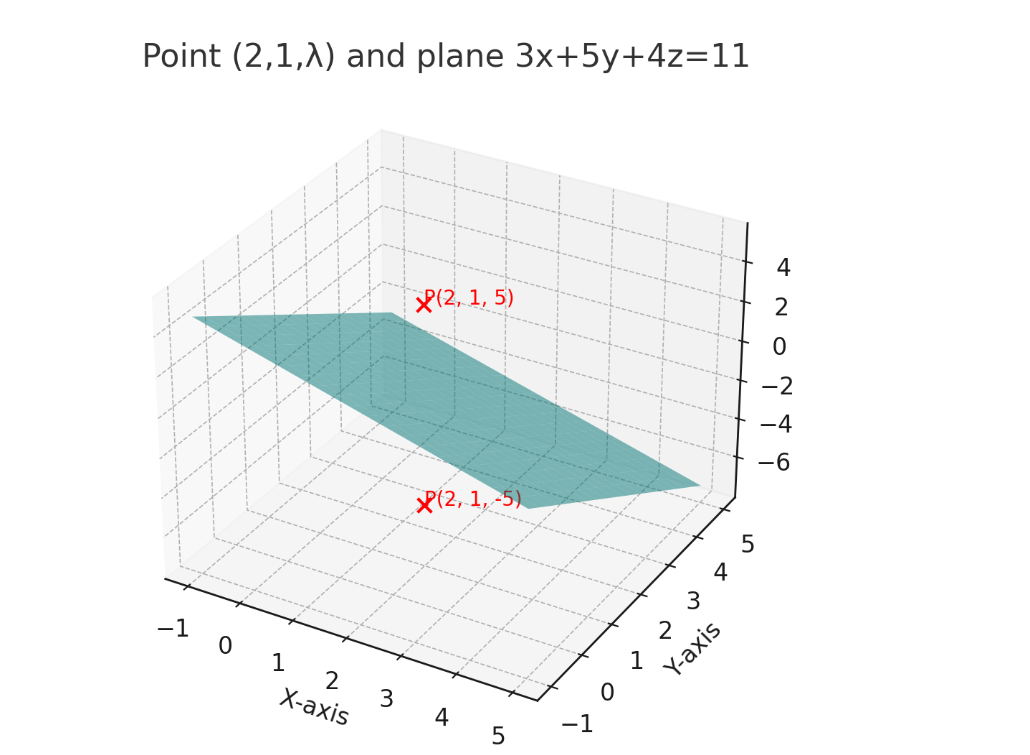
\includegraphics[width=0.90\linewidth]{figs/image.png}
    \caption{Image}
    \label{fig:placeholder}
\end{figure}


\end{document}